\documentclass[12pt,twoside,a4paper]{report}

\usepackage[utf8]{inputenc}
\usepackage[T1]{fontenc}


\usepackage{amsmath,amsfonts,amssymb}
\usepackage{graphicx}
\usepackage{float}
\usepackage[lined,boxed,commentsnumbered]{algorithm2e}

\title{Title to find ...}
\author{Gautier VAILLANT}

\begin{document}

\maketitle

\chapter*{Acknoledgements}

I would first like to gratefully thank Helmut Grubmüller and Bert De Groot for welcoming me in their lab. I also thank Carsten Kutzner who supervised my Internship. I also would like to Thank Bartosz Kohnke and Thomas Ullmann for providing me advice on my project.\\ 

Finally I would also like to thank Ivo Kabadschow and Andreas Beckmann who welcomed me in the Jülich Forschungszentrum to teach me the details of the FMM method. 

\chapter*{Abstract}

Simulating large pairwise interactions is a very important issue for Scientific research. It plays an important role in Astrophysics to know the dynamics of galaxies, in plasma physics or in our case in biophysics. This kind of simulations is typically with a complexity of $\mathcal{O}(N^2)$ which scales badly with the size of the system.

Some other techniques, such as the PME (Particle Mesh Ewald) and the FMM (Fast Multipole Method) are able to obtain a complexity of respectively $\mathcal{O}(N\log(N))$ qnd $\mathcal{O}(N)$.



\tableofcontents

\chapter*{Presentation of the Lab}

\chapter{Introduction to methods for computing electrostatic forces}


\section{$\mathcal{O}(N^2)$ method }

\subsection{Naive Method}

The coulombian interaction between two charged particles can be written the following way:

\begin{equation}
	\overrightarrow{F}_{A \rightarrow B} = \frac{q_A q_B \hat{r}_{AB} }{4\pi\epsilon_0|R_{AB}|^2}
	\label{coulombComplete}
\end{equation}

where $q_A $ and $q_B$ are respectively the charges of A and B, and $R_{AB}$ is the distance between $A$ and $B$.

In the thesis we will simplify the units of ~\eqref{coulombComplete} for computational reasons by just writing :

\begin{equation}
	\overrightarrow{F}_{A \rightarrow B} = \frac{q_A q_B \hat{r}_{AB} }{|R_{AB}|^2}
	\label{coulombSimplified}
\end{equation}

The first, naive way to compute electrostatic forces is the following : in order to compute the force acting on one particle, it is needed to obtain the coulombic interaction for each pair of particles.

So if we consider a set of $N$ charged particles, $N-1$ interactions are needed to compute the force acting on one specific particle. So in order to know the forces of the set of particles $N\cdot(N-1)$ operations are needed, hence an algorithmic complexity of $\mathcal{O}(N^2)$.

This gives the following algorithm:

\IncMargin{1em}
\begin{algorithm}[H]

\SetKwData{Left}{left}\SetKwData{This}{this}\SetKwData{Up}{up}
\SetKwData{Force}{force}

\SetKwFunction{ComputeForce}{computeForce}
\SetKwFunction{Union}{Union}\SetKwFunction{FindCompress}{FindCompress}
\SetKwInOut{Input}{input}\SetKwInOut{Output}{output}

\Input{A set of $N$ charged Particles}
\Output{A List of the forces\begin{equation}
	\overrightarrow{F}_{A \rightarrow B} = \frac{q_A q_B \hat{r}_{AB} }{|R_{AB}|^2}
	\label{coulombSimplified}
\end{equation} for each particle}
\BlankLine

\emph{For each particle i}\;
\For{$i\leftarrow 1$ \KwTo $N-1$}{
\emph{add interaction between particle $i$ and particle $j$ }\;
\For{$j\leftarrow i+1$ \KwTo $N$}{

	\Force$[i]$  $\leftarrow$ \Force$[i]$ + \ComputeForce{$i,j$}   \;

}
}
\caption{Naive method}\label{algo_disjdecomp}
\end{algorithm}\DecMargin{1em}


The complexity of such a computation limits its use to rather small systems and is not really usable for bigger systems.

\subsection{Possible improvements}

A possible improvement is to limit the interaction to a certain radius : if the distance between two particles if greater tham $R_0$, then the force is set to $0$.

So we have the following system :


\begin{equation}
  overrightarrow{F}_{A \rightarrow B}  =
	\begin{cases}
	  \frac{q_A q_B \hat{r}_{AB} }{|R_{AB}|^2}  & \text{if } R_{AB} < R_0 \\
	  \overrightarrow{0} & \text{otherwise}
	\end{cases}
\end{equation}

This technique est for example used for Lennard jones potentials, where the Intersity of the force is quickly decreasing. It allows to limit the number of interactions to only the close neighbours.\\

However, one of the problems of this optimisation, especially for long-range interactions such as coulombic int\begin{equation}
	\overrightarrow{F}_{A \rightarrow B} = \frac{q_A q_B \hat{r}_{AB} }{|R_{AB}|^2}
	\label{coulombSimplified}n_x*,
\end{equation}eractions is that using a cut-off can lead to artefacts : A particle feels the force, then crosses the cut-off radius. Suddenly, the particle doesn't feel any force anymore, thus the artefacts.

\begin{figure}[H]

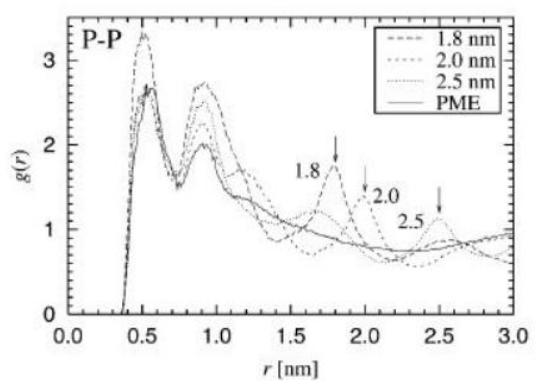
\includegraphics[scale=0.8]{artefact}
 \centering
 
\caption{Radial distribution function (RDF) $g(r)$ between the two
central atoms in the headgroup of a molecule: Cutoff distances are indicated by arrows. from ...}

\label{fig:artefact}

\end{figure}


As we can see in figure \ref{fig:artefact},  the radial distribution of the distance between two atom shows a peak, corresponding to the cutoff of the system. This shows that by using a cut-off technique we might see some artefacts.\\

So the two reasons we don't use a $\mathcal{O}(N^2)$ method is first because of its complexity, and unsing some optimization techniques can lead to artefacts.

\section{Fourier Transform-Based methods}

In this section, we will explain techniques using periodic boundary conditions and Fourier transformation in order to compute the potentials and the forces of the particles

\subsection{Ewald Summation}

This subset of techniques comes from a theoretical phycics technique called the Ewald summation.

Using periodic boundary conditions, the potential $V$ of one particle of the system is:

\begin{equation}
	V = \sum_{n_x^*,n_y^*,n_z^*} \sum_{i}^{N} \sum_{j}^{N} \frac{q_i q_j}{r_{ij}}
	\label{periodicSum}
\end{equation}

The equation \ref{periodicSum} is conditionnaly convergent and rather slow to converge. One technique discovered by ewald is to split the potential in two absolutely convergent terms :




\subsection{PME}

\section{Fast Summation methods}
	\subsection{Mathematical preliminaries}
	\subsection{Operators}
		\subsubsection{M2M}
		a
		\subsubsection{L2M}
		b
		\subsubsection{L2L}
		c


\chapter{Comparing FMM and PME accuracy}
\section{Presentation of GROMACS}
	\subsection{Structure of a File}
	\subsection{PME parameters}

\nocite{*}
\bibliographystyle{plain}
\bibliography{biblio} 



\end{document}

